\documentclass{beamer}

%% Encoding
%\usepackage[utf8]{inputenx} % Source code encoding (omitted with XeLaTeX/LuaLaTeX compilers)
%\usepackage[T1]{fontenc}    % PDF encoding (omitted with XeLaTeX/LuaLaTeX compilers)
\usepackage[final]{microtype}  % Improved typography
\usepackage[english]{babel}
%% Mathematics
\usepackage{amssymb}   % Extra symbols
\usepackage{amsthm}    % Theorem-like environments
\usepackage{thmtools}  % Theorem-like environments
\usepackage{mathtools} % Fonts and environments for mathematical formuale
\usepackage{mathrsfs}  % Script font with \mathscr{}
%% Miscellanous
\usepackage{graphicx}  % Tool for images
\usepackage{babel}     % Automatic translations
\usepackage{fvextra}   % For the csquotes package
\usepackage{csquotes}  % Quotes
\usepackage{textcomp}  % Extra symbols
\usepackage{listings}  % Typesetting code
\lstset{basicstyle = \ttfamily, frame = tb}
%% New commands for sets
\newcommand{\N}{\mathbb{N}}   % Natural numbers
\newcommand{\Z}{\mathbb{Z}}   % Integers
\newcommand{\Q}{\mathbb{Q}}   % Rational numbers
\newcommand{\R}{\mathbb{R}}   % Real numbers
\newcommand{\C}{\mathbb{C}}   % Complex numbers
\DeclareMathOperator{\mean}{mean}

%% Figures
\usepackage{graphicx} % To manage images
\usepackage{wrapfig}

%% TikZ for making figures
\usepackage{tikz}       % Package to make figures
\usepackage{wrapfig}
\usetikzlibrary{shapes,arrows,positioning,calc,automata, arrows.meta,positioning}
\usepackage{standalone} % for \includestandalone{tikzfile} %tikzfile.tex

%% Bibliography
\usepackage{mathscinet}
\usepackage[backend = biber, style = apa]{biblatex}
%\usepackage[backend = biber, style = chicago-authordate]{biblatex} % References as "Seborg et al."
%\usepackage[backend = biber, style = alphabetic]{biblatex} % References as [Seb+17]
\DeclareNameAlias{author}{family-given}
\addbibresource{sources.bib}
\usepackage{hyperref}

\usepackage{multicol}   % Multiple columns in slides and tables
\usepackage{tabularx}   % For big tables
\usepackage{verbatim}

\usepackage{minted}     % For code snippets

\setbeamertemplate{caption}{\raggedright\insertcaption\par} % To prevent prefix "Figure: Caption"


%Information to be included in the title page:
\title{This is a minimal LaTeX presentation}
\author{Author Name}
\date{June 2024}
 
 
 
\begin{document}

%%% Title page %%%
\frame{\titlepage}

\begin{frame}{For fancy OsloMet presentation}
    see \href{https://no.overleaf.com/latex/templates/oslomet-beamer-theme/wknwhwkrzvgk}{https://no.overleaf.com/latex/templates/oslomet-beamer-theme/wknwhwkrzvgk}
\end{frame}

\begin{frame}{Multicolumn slides}
    
\end{frame}

\begin{frame}
    Minipages can be used to place figures in rows and columns:
    \begin{figure}[ht]
        \begin{minipage}[t]{0.45\linewidth}
            \centering
            \caption{Top Left}
            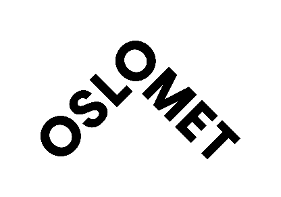
\includegraphics[width=0.75\textwidth]{figures/oslomet_logo.png}
            \label{fig:topleft}
        \end{minipage}
        \hspace{0.25cm}
        \begin{minipage}[t]{0.45\linewidth}
            \centering
            \caption{Top right}
            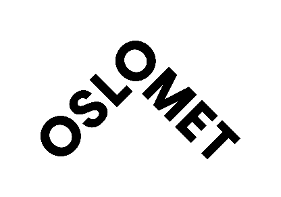
\includegraphics[width=0.75\textwidth]{figures/oslomet_logo.png}
            \label{fig:topright}
        \end{minipage}
        % New row (unless the minipage width is changed to e.g. 0.3\linewidth or 0.2\linewidth)
        \begin{minipage}[t]{0.45\linewidth}
            \centering
            \caption{Bottom left}
            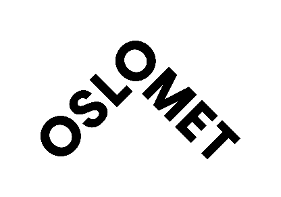
\includegraphics[width=0.75\textwidth]{figures/oslomet_logo.png}
            \label{fig:bottomleft}
        \end{minipage}
        \hspace{0.5cm}
        \begin{minipage}[t]{0.45\linewidth}
            \centering
            \caption{Bottom right}
            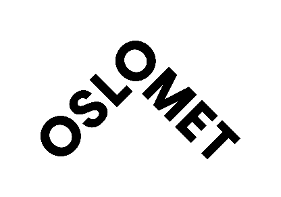
\includegraphics[width=0.75\textwidth]{figures/oslomet_logo.png}
            \label{fig:bottomright}
        \end{minipage}
    \end{figure}
\end{frame}

\begin{frame}{Referencing}
    Referencing can be done as usual with \texttt{\textbackslash cite\{citation-key\}}, e.g. \cite{winkler2018bdt}. Automatically add reference slides by using the following (remove \texttt{[allowframebreaks]} if the references fit on one page): \\
    
    
    \texttt{\textbackslash begin\{frame\}[allowframebreaks]\{Sources\}} \\
        \texttt{\textbackslash printbibliography} \\
    \texttt{\textbackslash end\{frame\}} 
\end{frame}


%\begin{frame}[allowframebreaks]{References}
\begin{frame}{References}
    \printbibliography
\end{frame}


\end{document}